\documentclass[11pt]{article}
% Author : liambeguin
%
% Usage :
%
% \documentclass[11pt]{article}
% % Author : liambeguin
%
% Usage :
%
% \documentclass[11pt]{article}
% % Author : liambeguin
%
% Usage :
%
% \documentclass[11pt]{article}
% \input{ets_page.tex}
% \EtsPageCourse{ELE778-01}
%	{Intelligence artificielle: r\'eseaux neuroniques et syst\`emes experts}
% \EtsPageTitle{Laboratoire 2}
% \EtsPageProf{Cynthia}{Moussa}
% \EtsPageAuthA{Liam}{Beguin}{BEGL02129304}
% \EtsPageAuthB{Louis}{Laporte}{LAPL14128903}
% \EtsPageAuthC{}{}{}
%
% \begin{document}
% \MakeEtsPage
% \end{document}

\usepackage[french]{babel}
\usepackage[utf8]{inputenc}
\usepackage{tikz}
\usepackage{pgf}
\usetikzlibrary{arrows,automata}
\usepackage[left=2cm, right=2cm]{geometry}
\usepackage{amsmath,amsfonts,amssymb}
\usepackage{listings}

\newcommand{\EtsPageCourse}[2]{\renewcommand{\EtsPageCourse}{
	\textsc{\textbf{\Huge #1 - #2}}
}}
\newcommand{\EtsPageTitle} [1]{\renewcommand{\EtsPageTitle}{
	\textsc{\Large #1 }
}}
\newcommand{\EtsPageProf}  [2]{\renewcommand{\EtsPageProf}{
			\textsc{\Large Pr\'esent\'e \`a : \\
			#1 \textsc{#2}}
}}
\newcommand{\EtsPageAuthA} [3]{\renewcommand{\EtsPageAuthA}{
	\large #1 \textsc{#2} \\\emph{#3}
}}
\newcommand{\EtsPageAuthB} [3]{\renewcommand{\EtsPageAuthB}{
	\large #1 \textsc{#2} \\\emph{#3}
}}
\newcommand{\EtsPageAuthC} [3]{\renewcommand{\EtsPageAuthC}{
	\large #1 \textsc{#2} \\\emph{#3}
}}

\newcommand{\HRule}{\rule{\linewidth}{0.5mm}}

\newcommand{\EtsPageGenerate}{
	\begin{titlepage}
		\begin{center}
			\vspace{5cm}
			\EtsPageCourse
			\vspace{2cm}

			\EtsPageTitle
			\vspace{2.5cm}

			\EtsPageProf
			\vspace{1.5cm}

			% Bottom of the page
			\vfill
			% Authors
			\begin{minipage}{0.4\textwidth}
				\begin{flushleft}
					\EtsPageAuthA
				\end{flushleft}
			\end{minipage}
			\begin{minipage}{0.4\textwidth}
				\begin{flushright}
					\EtsPageAuthB
				\end{flushright}
			\end{minipage}
			\begin{minipage}{0.4\textwidth}
				\begin{center}
					\EtsPageAuthC
				\end{center}
			\end{minipage}

			\vspace{2cm}
			\HRule \\[0.4cm]
			{ \huge \bfseries \'Ecole de technologie superieure \\[0.4cm] }
			\HRule \\[1.5cm]
			\vspace{1.5cm}

			%date
			{\large \today}
		\end{center}
	\end{titlepage}
}

% \EtsPageCourse{ELE778-01}
%	{Intelligence artificielle: r\'eseaux neuroniques et syst\`emes experts}
% \EtsPageTitle{Laboratoire 2}
% \EtsPageProf{Cynthia}{Moussa}
% \EtsPageAuthA{Liam}{Beguin}{BEGL02129304}
% \EtsPageAuthB{Louis}{Laporte}{LAPL14128903}
% \EtsPageAuthC{}{}{}
%
% \begin{document}
% \MakeEtsPage
% \end{document}

\usepackage[french]{babel}
\usepackage[utf8]{inputenc}
\usepackage{tikz}
\usepackage{pgf}
\usetikzlibrary{arrows,automata}
\usepackage[left=2cm, right=2cm]{geometry}
\usepackage{amsmath,amsfonts,amssymb}
\usepackage{listings}

\newcommand{\EtsPageCourse}[2]{\renewcommand{\EtsPageCourse}{
	\textsc{\textbf{\Huge #1 - #2}}
}}
\newcommand{\EtsPageTitle} [1]{\renewcommand{\EtsPageTitle}{
	\textsc{\Large #1 }
}}
\newcommand{\EtsPageProf}  [2]{\renewcommand{\EtsPageProf}{
			\textsc{\Large Pr\'esent\'e \`a : \\
			#1 \textsc{#2}}
}}
\newcommand{\EtsPageAuthA} [3]{\renewcommand{\EtsPageAuthA}{
	\large #1 \textsc{#2} \\\emph{#3}
}}
\newcommand{\EtsPageAuthB} [3]{\renewcommand{\EtsPageAuthB}{
	\large #1 \textsc{#2} \\\emph{#3}
}}
\newcommand{\EtsPageAuthC} [3]{\renewcommand{\EtsPageAuthC}{
	\large #1 \textsc{#2} \\\emph{#3}
}}

\newcommand{\HRule}{\rule{\linewidth}{0.5mm}}

\newcommand{\EtsPageGenerate}{
	\begin{titlepage}
		\begin{center}
			\vspace{5cm}
			\EtsPageCourse
			\vspace{2cm}

			\EtsPageTitle
			\vspace{2.5cm}

			\EtsPageProf
			\vspace{1.5cm}

			% Bottom of the page
			\vfill
			% Authors
			\begin{minipage}{0.4\textwidth}
				\begin{flushleft}
					\EtsPageAuthA
				\end{flushleft}
			\end{minipage}
			\begin{minipage}{0.4\textwidth}
				\begin{flushright}
					\EtsPageAuthB
				\end{flushright}
			\end{minipage}
			\begin{minipage}{0.4\textwidth}
				\begin{center}
					\EtsPageAuthC
				\end{center}
			\end{minipage}

			\vspace{2cm}
			\HRule \\[0.4cm]
			{ \huge \bfseries \'Ecole de technologie superieure \\[0.4cm] }
			\HRule \\[1.5cm]
			\vspace{1.5cm}

			%date
			{\large \today}
		\end{center}
	\end{titlepage}
}

% \EtsPageCourse{ELE778-01}
%	{Intelligence artificielle: r\'eseaux neuroniques et syst\`emes experts}
% \EtsPageTitle{Laboratoire 2}
% \EtsPageProf{Cynthia}{Moussa}
% \EtsPageAuthA{Liam}{Beguin}{BEGL02129304}
% \EtsPageAuthB{Louis}{Laporte}{LAPL14128903}
% \EtsPageAuthC{}{}{}
%
% \begin{document}
% \MakeEtsPage
% \end{document}

\usepackage[french]{babel}
\usepackage[utf8]{inputenc}
\usepackage{tikz}
\usepackage{pgf}
\usetikzlibrary{arrows,automata}
\usepackage[left=2cm, right=2cm]{geometry}
\usepackage{amsmath,amsfonts,amssymb}
\usepackage{listings}

\newcommand{\EtsPageCourse}[2]{\renewcommand{\EtsPageCourse}{
	\textsc{\textbf{\Huge #1 - #2}}
}}
\newcommand{\EtsPageTitle} [1]{\renewcommand{\EtsPageTitle}{
	\textsc{\Large #1 }
}}
\newcommand{\EtsPageProf}  [2]{\renewcommand{\EtsPageProf}{
			\textsc{\Large Pr\'esent\'e \`a : \\
			#1 \textsc{#2}}
}}
\newcommand{\EtsPageAuthA} [3]{\renewcommand{\EtsPageAuthA}{
	\large #1 \textsc{#2} \\\emph{#3}
}}
\newcommand{\EtsPageAuthB} [3]{\renewcommand{\EtsPageAuthB}{
	\large #1 \textsc{#2} \\\emph{#3}
}}
\newcommand{\EtsPageAuthC} [3]{\renewcommand{\EtsPageAuthC}{
	\large #1 \textsc{#2} \\\emph{#3}
}}

\newcommand{\HRule}{\rule{\linewidth}{0.5mm}}

\newcommand{\EtsPageGenerate}{
	\begin{titlepage}
		\begin{center}
			\vspace{5cm}
			\EtsPageCourse
			\vspace{2cm}

			\EtsPageTitle
			\vspace{2.5cm}

			\EtsPageProf
			\vspace{1.5cm}

			% Bottom of the page
			\vfill
			% Authors
			\begin{minipage}{0.4\textwidth}
				\begin{flushleft}
					\EtsPageAuthA
				\end{flushleft}
			\end{minipage}
			\begin{minipage}{0.4\textwidth}
				\begin{flushright}
					\EtsPageAuthB
				\end{flushright}
			\end{minipage}
			\begin{minipage}{0.4\textwidth}
				\begin{center}
					\EtsPageAuthC
				\end{center}
			\end{minipage}

			\vspace{2cm}
			\HRule \\[0.4cm]
			{ \huge \bfseries \'Ecole de technologie superieure \\[0.4cm] }
			\HRule \\[1.5cm]
			\vspace{1.5cm}

			%date
			{\large \today}
		\end{center}
	\end{titlepage}
}


\usepackage{graphicx}
\usepackage{multirow}
\usepackage{color, colortbl}
\usepackage[
	pdftitle   ={ELE778 rapport de laboratoire 3.2},
	pdfsubject ={Detail de l'implementation d'un reseau de type Learning
				Vector Quantization},
	pdfauthor  ={Liam BEGUIN - Louis LAPORTE},
	pdfkeywords={LVQ, OLVQ, Centroid, TiDigits classification},
]{hyperref} % Required for links
\usepackage{enumitem}


\EtsPageCourse{ELE778-01}
	{Intelligence artificielle: r\'eseaux neuroniques et syst\`emes experts}
\EtsPageTitle{Laboratoire 3}
\EtsPageProf{Cynthia}{Moussa}
\EtsPageAuthA{Liam}{Beguin}{BEGL02129304}
\EtsPageAuthB{Louis}{Laporte}{LAPL14128903}
\EtsPageAuthC{}{}{}

\begin{document}
\EtsPageGenerate
\tableofcontents

\newpage
\section{Introduction}
Lors du laboratoire 2 nous avons impl\'ement\'e un r\'eseau de neurone \`a
r\'etro-propagation du gradient d’erreur. Pour ce laboratoire nous allons
r\'eutilliser l'étape de pré-traitement et nous allons implémenter un r\'eseau
de neurones de type LVQ (Learning Vector Quantization) dans le but de
classifier, le plus précisément possible, le dataset {\em TiDigits} (english
spoken digits from 1 to 9). Enfin, nous comparerons les 2 types
d'impl\'ementation quand a leur erreur hors echantillon et leur temps
d'apprentissage.

Pour implémenter ce r\'eseau de neurones, nous utiliserons {\em Python}.
Voici une liste d'avantages versus inconv\'enients qui ont motiv\'e notre choix
pour ce language :
\begin{itemize}
	\item Avantages:
		\subitem Rapidit\'e de d\'eveloppement,
		\subitem Language interpr\'et\'e donc pas de compilation,
		\subitem Modules de calcul matriciel performants,
		\subitem Language accessible,
	\item Inconvenients:
		\subitem Language interpr\'et\'e donc moins rapide. \\
\end{itemize}

Dans un premier temps, nous entrainerons le r\'eseau sur un set de donn\'ees puis
nous \'evaluerons sa capacit\'e a g\'en\'eraliser sur de nouvelles donn\'ees
non utilis\'ees lors de l'entrainement.

\section{Impl\'ementation du r\'eseau de neurones}
\subsection{Architecture globale}
\begin{figure}[htp]
	\centering
	
\includegraphics[scale=.5]{img/tesselation.png}
	\caption{Repr\'esentation d'une classification de type dans $\mathbb{R}^2$.}
\end{figure}

Comme dit en introduction, nous allons impl\'ementer un r\'eseau de neurones
de type LVQ. Le LVQ est un algorithme supervis\'e dit comp\'etitif dans le sens
o\`u les sorties com\'petitionnent afin de ne donner qu'une seule sortie active. 

Le LVQ est une m\'ethode de classification o\`u chaque sortie repr\'esente une
classe, le nombre de classes doit cependant etre fournit par l'utilisateur.
Au cours du processus d'apprentissage les poids (ou prototypes ou encore
codebooks) de chaque classe sont attir\'es ou repouss\'es
dans le but de les positionner optimalement par rapport aux donn\'ees
d'entrainement.


\paragraph{Actualisation des poids:} Les poids sont mis \`a jour  \`a l'aide
de expression suivante:\\
\begin{equation}
	\begin{aligned}
		{\bf w}_j (t+1) &= {\bf w}_j (t) + s(t) \cdot \eta\cdot
		\big({\bf x} - {\bf w}_j (t)\big)\\
	\end{aligned}
\end{equation}
O\`u: 
\begin{equation}
	\left\{
	\begin{aligned}
		j &= \text{{\em numero} de la classe,} \\ t &= \text{instant ou epoch} \\
		s &= 1 \text{ si } {\hat y} = y \text{ sinon } s= -1\\
		\eta &= \text{taux d'apprentissage}
	\end{aligned}
	\right .
\end{equation}

\subsection{Extraction des donn\'ees}
\begin{figure}[h]
	\centering
	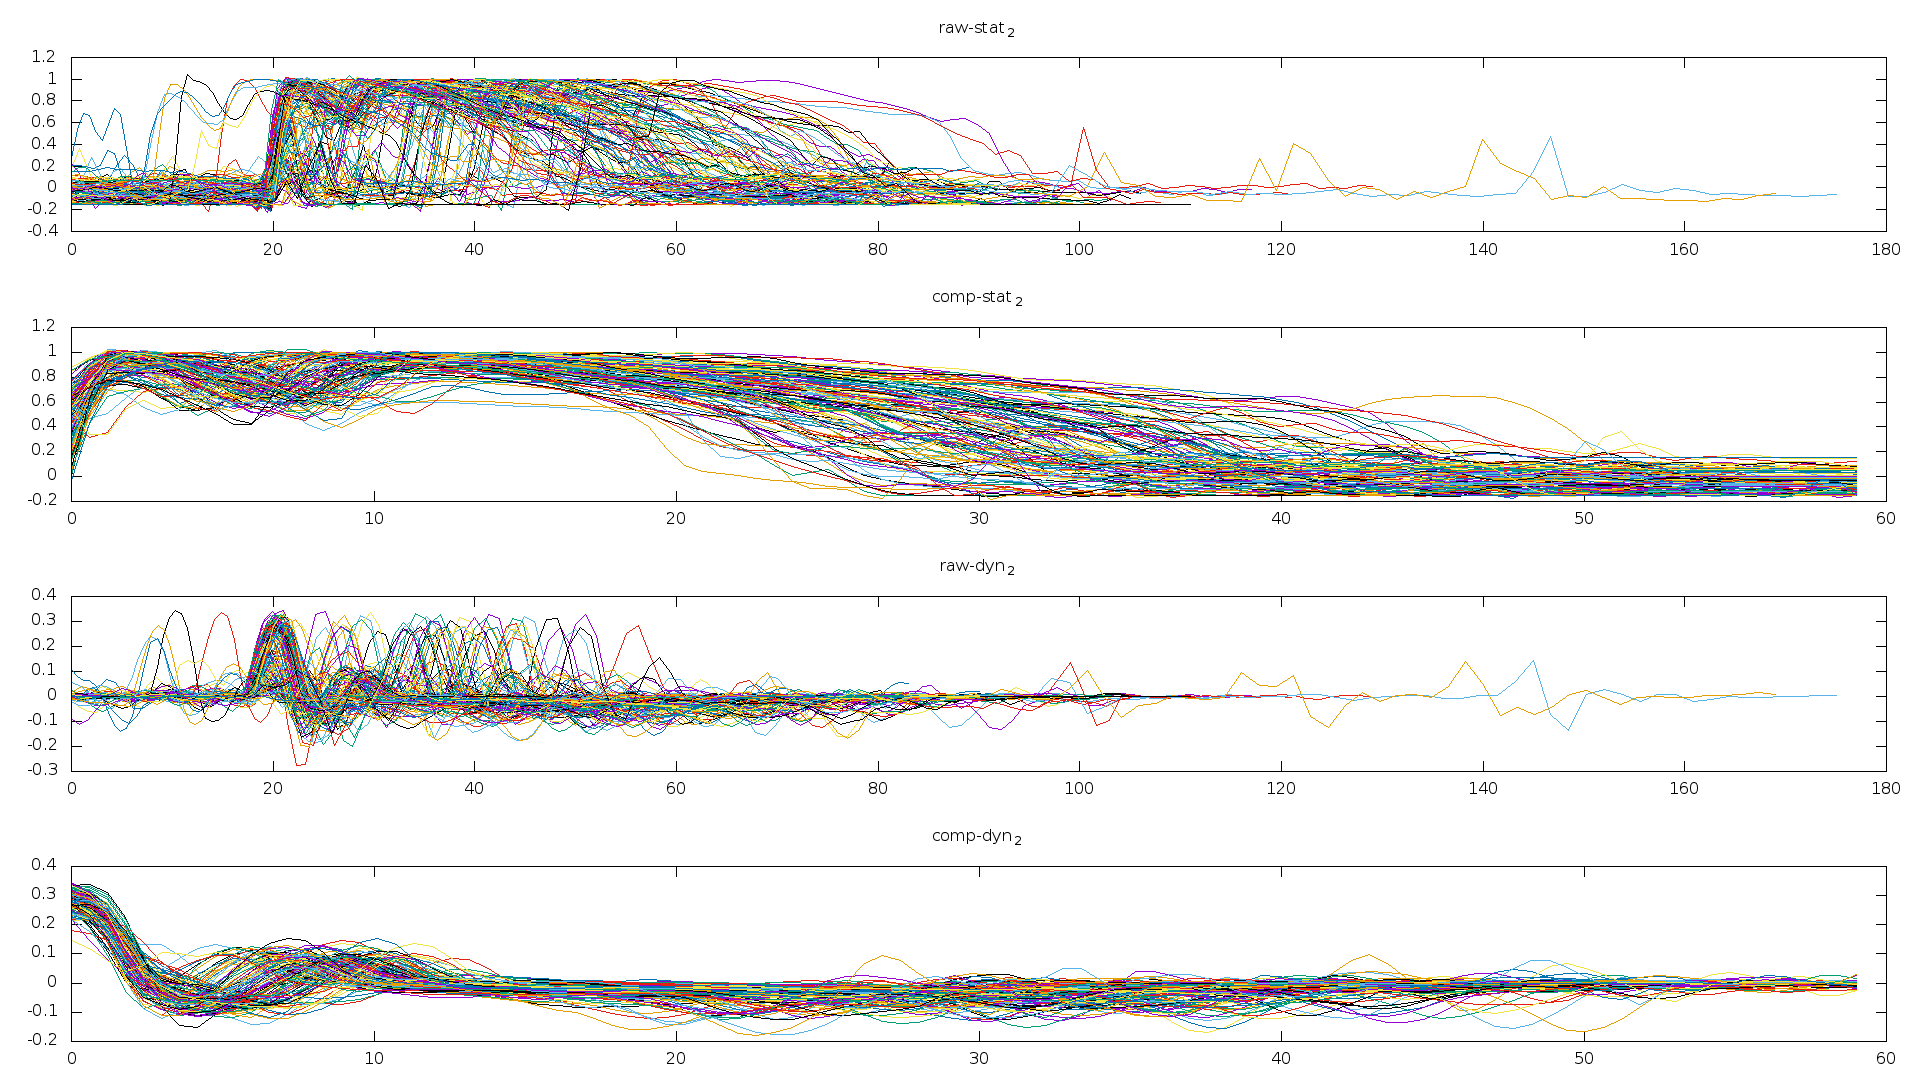
\includegraphics[scale=.3]{img/preprocessing.png}
	\caption{Repr\'esentation des \'en\'ergies statiques et dynamiques avant et
	apr\`es le traitement}
\end{figure}

Pour extraire les informations de la base de donn\'ee {\em TiDigits}, nous
avons utilis\'e le code que nous avions d\'evelopp\'e pour la premi\`ere
partie du laboratoire.
Nous nous sommes bas\'es sur les similarit\'es entre la prononciation d'un
m\^eme chiffre par plusieurs individus. Pour cela, nous avons filtr\'e
les \'energies statiques et dynamiques afin de pouvoir accentuer les
propri\'et\'es de chaque chiffre.


Le filtrage consiste dans un premier temps \`a utiliser une op\'eration de
seuillage sur l'\'energie statique afin de d\'et\'ecter le d\'ebut du mot et
d'\'eliminer tout le {\em blanc} qui se trouve au d\'ebut de l'enregistrement.
La seconde \'etape permet d'aligner le d\'ebut de chaque mot en utilisant le
premier maximum de l'\'energie dynamique.
Ceci nous permet de ne pas \^etre trop sensible aux diff\'erences d'attaque
entre les individus.

Comme tous les fichiers n'ont pas la m\^eme taille, nous devons ajouter
du padding afin que les donn\'ees puissent \^etre utilis\'ees comme
entr\'ee pour le r\'eseau. En effet, dans le cas o\`u les longueurs ne sont pas
identiques, il est impossible d'alimenter le r\'eseau en raison d'erreurs
de dimensions sur les produits matriciels.
D'autre part, dans le but d'am\'eliorer la vitesse de convergence de
l'apprentissage et de limiter la complexit\'e du mod\`ele, nous avons choisi de
ne garder que les donn\'ees statiques et de les normaliser, selon chaque colonne.

La fonction d'extraction des donn\'ees {\em extract\_datasets()}
est con\c{c}ue pour prendre 2 param\`etres: le nombre de features d\'esir\'e
(40, 50, 60, ...) et un bool\'een permettant de choisir si l'on desir ou non
classifier selon le sexe de l'interpr\`ete. cette fonction retourne 3 listes:
un {\em training\_set}, un {\em validation\_set} et un {\em test\_set} o\`u
chaque \'el\'ement est une combinaison de 2 vecteurs les features {\bf x} et
les labels {\bf y}.

Nous avons pour ce nouvel algorithme ajouter une option permettant de fournir
des labels sous forme non-vectoris\'es afin de faciliter le traitement lors des
\'etapes suivantes.



\subsection{Initialisation du r\'eseau}
Lorsque le r\'eseau est instanci\'e, nous passons le nombre de centro{\"i}de que
nous voulons par classe.
Ensuite nous avons le choix entre 2 types d'initialisation de poids.\\
Le premier choix permet d'initialiser en choisissant des \'echantillons de test
de mani\`ere al\'etoire parmis le dataset.

La seconde m\'ethode permet de choisir les prototypes initiaux en calculant le
centro\"ide de l'ensemble des points du training set pour chaque classe.

\lstset{tabsize = 4,
frame=lines,
numbers=left,
captionpos=b,
caption = {Initialisation des poids avec la m\'ethode de selection al\'eatoire},
language = python,
basicstyle=\small}
\begin{lstlisting}
def random_weight_init(input_size, output_size, ppc, tr_d):
    """ select codebooks at random within the dataset """

    weights = [ np.zeros(shape=(input_size, 1)) ] * (output_size * ppc)

    np.random.shuffle(tr_d)
    tr_dX = []
    tr_dY = []
    for x, y in tr_d:
        tr_dX.append(x)
        tr_dY.append(y)

    tr_dX = np.array(tr_dX)
    tr_dY = np.array(tr_dY)

    for w_idx, w in enumerate(weights):
        match = np.where(tr_dY == w_idx%output_size)[0][0]
        weights[w_idx] = tr_dX[match]

    return weights
\end{lstlisting}

\lstset{tabsize = 4,
frame=lines,
numbers=left,
captionpos=b,
caption = {Initialisation des poids avec la m\'ethode des centres},
language = python,
basicstyle=\small}
\begin{lstlisting}
def average_weight_init(input_size, output_size, ppc, tr_d):
    """ init codebooks using the mean point """

    weights = [ np.zeros(shape=(input_size, 1)) ] * (output_size * ppc)

    np.random.shuffle(tr_d)
    tr_dX = []
    tr_dY = []
    for x, y in tr_d:
        tr_dX.append(x)
        tr_dY.append(y)

    tr_dX = np.array(tr_dX)
    tr_dY = np.array(tr_dY)

    for w_idx, w in enumerate(weights):
        match = np.where(tr_dY == w_idx%output_size)
        weights[w_idx] = np.mean(tr_dX[match], axis=0)

    return weights
\end{lstlisting}
\newpage



\paragraph{Validation crois\'ee:} Pour \'evaluter l'erreur commise sur des
\'echantillons jamais vu auparavant, il est
important de s\'eparer le set de donn\'ees en deux une partie pour l'entrainement
l'autre pour la validation. Plusieurs m\'ethodes diff\'erentes sont disponibles
pour d\'eterminer comment s\'eparer le dataset. Plus on \`a de donn\'ees dans le set
d'entrainement plus la pr\'ediction sera bonne mais moins on sera capable de
quantifier la capacit\'e de g\'en\'eralisation du r\'eseau et inversement.

Une m\'ethode int\'eressante \`a citer est le \href{http://work.caltech.edu/slides/slides13.pdf}
{\emph{V-folds} ou \emph{K-folds}} qui permet de maximiser le nombre d'\'echantillons
d'entrainement en divisant le set complet en $V$ sous ensembles. Le r\'eseau est
ensuite entrain\'e sur tous les sous-ensembles moins un qui est utilis\'e pour la
validation (le sous-ensemble de validation est choisi al\'eatoirement et change
\`a chaque \'epoque d'apprentissage). Il faut noter qu'il est important de
s\'electionner les \'echantillons de mani\`ere al\'eatoire afin de ne pas biaiser
l'apprentissage du r\'eseau.

Cependant, notre set de donn\'ees \'etant d\'ej\`a s\'epar\'e en plusieurs sous-ensembles,
nous garderons ces m\'ethodes comme pistes d'am\'elioration futures.

\paragraph{Le early stopping} est utilis\'e ici aussi mais dans un autre but.
N'ayant plus de {\em sur-apprentissage}, il consiste simplement \`a monitorer
les erreurs au cours de l'entrainement du r\'eseau et
de l'interrompre sous certaines conditions de seuil.

\newpage
\subsection{Entrainement}
Lors de l'entrainement on passe comme param\`etre le nombre maximal d'epochs,
le taux d'apprentissage $\eta$ et $\eta\_decay$, un booleen activant ou non la
diminution du taux d'apprentissage.
L'entrainement du r\'eseau est un processus gourmand en calculs et demandant
beaucoup de ressources. Il est donc important de bien l'optimiser.



\lstset{tabsize = 4,
frame=lines,
numbers=left,
captionpos=b,
caption = {Definition de notre methode d'apprentissage},
language = python,
basicstyle=\small}
\begin{lstlisting}
def train(self, tr_d, eta, epochs, eta_decay=False, va_d=None, estop=True):
	
	va_err, tr_err = [], []
	for i in xrange(0, epochs):
		for x, y in tr_d:
		    d = []
		    for w in self.weights:
		        # Compute distances
		        d.append(self.distance(x, w))

		    # find closest centroid
		    bmu = np.argmin(d)
		    # Update closest weight: Best Matching Unit
		    if bmu % self.output_size == y: 
		    	s = 1
		    else: 
		    	s = -1
		    self.weights[bmu] += s * eta * (x - self.weights[bmu])
		    
		if eta_decay:
            # Compute optimized learning rate
            eta = eta / (1 + s * eta) if eta < 1 else 1
            
        tr_err.append(self.eval_error_rate(tr_d))
        # Validation
        if va_d:
            va_err.append(self.eval_error_rate(va_d))
            # Stop early if validation error is very low
            if estop and va_err[-1] < 0.01: break

        self.learn_time = datetime.datetime.now() - self.learn_time
        
        return tr_err, va_err
\end{lstlisting}

\newpage
\subsection{Ajustement des hyper-param\`etres}
\begin{table}[h]
	\centering
	\begin{tabular}{|c|c|c|c|c|c|c|c|c|c|c|c|c|c|}
		\hline
		dataset & out  & $\eta$ & $\eta\_decay$ & epoch  & proto  & tr(\%) & va(\%) & test(\%) & t(s)\\
		\hline		
		40	& 18 & 0.1 & True & 6 & 10 & 3.4 & 0.9 & 9.9 & 20\\
		\hline
		\rowcolor{green}		
		40	& 18 & 0.5 & True & 10 & 10 & 2.8 & 5.5 & 8.4 & 29\\
		\hline		
		40	& 18 & 0.6 & True & 10 & 10 & 3.6 & 3.7 & 9.7 & 29\\
		\hline		
		40	& 18 & 0.5 & True & 20 & 20 & 1.7 & 6.5 & 8.8 & 112\\
		\hline		
		40	& 18 & 0.1 & True & 20 & 20 & 2.9 & 2.7 & 10.2 & 112\\
		\hline		
		40	& 18 & 0.01 & True & 20 & 20 & 6.6 & 3.7 & 12.7 & 121\\
		\hline		
		40	& 18 & 0.1 & False & 20 & 20 & 4.8 & 0.9 & 10.7 & 121\\
		\hline		
		40	& 9 & 0.1 & True & 1 & 20 & 4.0 & 0 & 5.7 & 3\\
		\hline		
		40	& 9 & 0.5 & True & 2 & 20 & 2.2 & 0 & 4.3 & 6\\
		\hline
		40	& 9 & 0.6 & True & 2 & 20 & 2.3 & 0 & 4.3 & 6\\
		\hline
		\rowcolor{green}
		40	& 9 & 0.5 & True & 2 & 21 & 2.4 & 0.9 & 3.2 & 7\\
		\hline
		50  & 9 & 0.5 & True & 2 & 21 & 2.4 & 0.9 & 3.2 & 7\\
		\hline
		60  & 9 & 0.5 & True & 20 & 21 & 2.4 & 0.9 & 3.2 & 38\\
		\hline
\end{tabular}
  \caption{Tableau r\'ecapitalif des tests effectu\'es sur les
	hyper-param\`etres sur un {\em i5 dual-core, 2.2GHz} pour le LVQ }
\end{table}


Pour obtenir la meilleur solution nous avons cherch\'e en premier lieu le
taux d'apprentissage $\eta$  qui donnait la plus petite erreur sur le training
set, ensuite nous avons ajust\'e le nombre de prototype par classe avec et sans
la r\'eduction du taux d'apprentissage. Nous pouvons conclure qu'aux vues des
r\'esultats la meilleur configuration est pour un dataset contenant de 40
\'el\'ements avec un taux d'apprentissage de $0.5$.
Lorsque nous avons fait la classification homme/femme, nous avons observ\'e
qu'\'a partir de 10 prototypes (par classe) les performances sur le taux
d'erreur du dataset de test n'\'etait pas am\'elior\'ees.

En ce qui concerne la classification des chiffres uniquement le choix
du nombre de prototypes est le meilleur entre 21 et 22, avant ou apr\`es les
valeurs les performances se d\'egradent.
\newpage

\subsection{Inspection du res\'eau}
Parmis les contraintes obligatoires, il nous est aussi demand\'e de pouvoir
inspecter les couches cach\'ees du r\'eseau. Pour ce faire, nous tirons parti du
fait que {\em Python} est un language interpr\'et\'e et qu'il fournit \`a
l'utilisateur une interface int\'eractive(c.f. laboratoire 2.2).

En combinaison avec la possibilit\'e de sauvegarder l'\'etat des
objects {\em LVQ} sous la forme de fichiers (compress\'es ou non), nous
pouvons ais\'ement analyser chaque couche.




\section{Discussions}
\subsection{Comparaison LVQ vs MLP}
\begin{table}[h]
	\centering
	\begin{tabular}{|c|c|c|c|c|c|c|c|c|c|c|c|c|c|}
		\hline
		dataset & out & $\sigma$  & cost & $\Omega$ & $\eta$ & $\lambda$ &
			epoch  & batch & hidden & tr(\%) & va(\%) & test(\%) & t(s)\\
		\hline		
		40	& 18 & s & C & L2 & 0.5 & 0.001 & 30 & 10 & 0 & 0 & 2 & 14 & 20 \\
		\hline
		40	& 9 & s & C & L2 & 0.5 & 0.001 & 30 & 10 & 0 & 1 & 1 & 7 & 20 \\
		\hline
\end{tabular}
  \caption{Tableau r\'ecapitalif des tests effectu\'es sur les
	hyper-param\`etres sur un {\em i5 dual-core, 2.2GHz} pour le MLP }
\end{table}
\begin{table}[h]
	\centering
	\begin{tabular}{|c|c|c|c|c|c|c|c|c|c|c|c|c|c|}
		\hline
		dataset & out  & $\eta$ & $\eta_{decay}$ & epoch  & proto  & tr(\%)
		& va(\%) & test(\%) & t(s)\\
		\hline		
		40	& 18 & 0.5 & True & 10 & 10 & 2.8 & 5.5 & 8.4 & 29\\
		\hline
		40	& 9 & 0.5 & True & 2 & 21 & 2.4 & 0.9 & 3.2 & 7\\
		\hline
\end{tabular}
  \caption{Tableau r\'ecapitalif des tests effectu\'es sur les
	hyper-param\`etres sur un {\em i5 dual-core, 2.2GHz} pour le LVQ }
\end{table}

Nous pouvons constat\'e qu'avec le {\em LVQ} nous avons de meilleure
performance sur le dataset de test et en moins d'epochs. Il faut cependant
noter que pour le {\em MLP}, une fois que les param\`etres donnant les
meilleurs performances sont trouv\'ees il n'y a plus besoin de les modifier si
on change le nombre d'entr\'ee. De plus les temps de calcul pour trouver les
meilleurs r\'eponses
sont identiques alors que pour le {\em LVQ} il est n\'ecessaire de changer les
param\`etres. Le temps de calcul augmente par 4 fois entre 9 et 18 entr\'ees pour
le {\em LVQ}. On peut en clonclure que le {\em MLP} est plus flexible quant au
nombre d'entr\'ee mais a de moins bonne performance sur la dataset de test. Le
{\em LVQ} est plus performant mais lorsqu'on augmente le nombre de d'entr\'ee il devient
plus lent.
Le {\em LVQ} est donc plus rapide pour nombre d'entr\'ees limit\'ees et fixes
tandis que le {\em MLP} est plus g\'en\'erique.

\subsection{Conclusion et pistes d'am\'elioration}
Encore une fois, du a un manque de temps, nous n'avons pas pouss\'e plus que
necessaire sur les optimisations de type (convertion des listes de np.array en
matrices). Ceci permettrai certainement de rendre le syst\`eme un peu plus
rapide.

En revanche, malgr\'e cela, on observe tout de m\^eme de bonnes performances.
On remarque aussi une bonne capacit\'e de g\'en\'eralisation avec une erreur
d'environs 5-10\% sur le set de test apr\`es l'apprentissage.

Ici aussi, nous avons impl\'ement\'e la g\'en\'eration des matrices de confusion.
En les observant attentivement, on remarque que le r\'eseau commet
principalement des erreurs lors de la classification homme/femme. Ceci pourrait
probablement \^etre du \`a un pr\'e-traitement trop {\em agressif} ou encore \`a
un manque d'\'echantillons d'entrainement. Cette classification erron\'ee
pourrait peut-\^etre \^etre ajust\'ee en impl\'ementant une m\'ethode de
validation-crois\'ee plus avanc\'ee telle que le {\em V-folds}
cit\'e pr\'ec\'edemment.

D'autres pistes d'am\'eliorations seraient d'impl\'ementer un ajustement dynamique
du nombre de prototypes par classes ou encore d'implementer des variantes du
{\em LVQ} plus performantes telles que le
\href{http://www.cis.hut.fi/research/lvq_pak/lvq_doc.txt}{{\em LVQ2}, {\em LVQ3}}
ou encore le {\em DVQ}.
On pourrait aussi penser \`a combiner plusieurs types de r\'eseaux (c.f. {\em DTW})
en utilisant des methodes \href{http://work.caltech.edu/slides/slides18.pdf}{d'agr\'egation}. 


\end{document}
% vim: cc=80 :
